\documentclass[10pt]{article}
%%%%%%%%%%%%%%%%%%%%%%%%%
%			AZ' STANDARD NEWCOMMANDS
%%%%%%%%%%%%%%%%%%%%%%%%%
\usepackage[applemac]{inputenc}
\usepackage[english]{babel}
\usepackage[T1]{fontenc}
\usepackage{cite, url,color} % Citation numbers being automatically sorted and properly "compressed/ranged".
%\usepackage{pgfplots}
\usepackage{graphics,amsfonts}
\usepackage[pdftex]{graphicx}
\usepackage[cmex10]{amsmath}
% Also, note that the amsmath package sets \interdisplaylinepenalty to 10000
% thus preventing page breaks from occurring within multiline equations. Use:
 \interdisplaylinepenalty=2500
% after loading amsmath to restore such page breaks as IEEEtran.cls normally does.

%% Useful packages for creation of two-column and more complex figures
% Compact lists
\usepackage{enumitem}
\usepackage{booktabs}
\usepackage{fancyvrb}

\usepackage{listings} % inserisce listati di programmi
\definecolor{commenti}{rgb}{0.13,0.55,0.13}
\definecolor{stringhe}{rgb}{0.63,0.125,0.94}
\lstloadlanguages{Matlab}
\lstset{% general command to set parameter(s)
framexleftmargin=0mm,
frame=single,
keywordstyle = \color{blue},% blue keywords
identifierstyle =, % nothing happens
commentstyle = \color{commenti}, % comments
stringstyle = \ttfamily \color{stringhe}, % typewriter type for strings
showstringspaces = false, % no special string spaces
emph = {for, if, then, else, end},
emphstyle = \color{blue},
firstnumber = 1, % numero della prima linea
numbers =right, %  show number_line
numberstyle = \tiny, % style of number_line
stepnumber = 5, % one number_line after stepnumber
numbersep = 5pt,
language = {Matlab}, % per riconoscere la sintassi matlab
extendedchars = true, % per abilitare caratteri particolari
breaklines = true, % per mandare a capo le righe troppo lunghe
breakautoindent = true, % indenta le righe spezzate
breakindent = 30pt, % indenta le righe di 30pt
basicstyle=\footnotesize\ttfamily
}

%Pseudocode package
\usepackage{algorithm}
\usepackage[noend]{algpseudocode}

\usepackage{array}
% http://www.ctan.org/tex-archive/macros/latex/required/tools/
\usepackage{mdwmath}
\usepackage{mdwtab}
%mdwtab.sty	-- A complete ground-up rewrite of LaTeX's `tabular' and  `array' environments.  Has lots of advantages over
%		   the standard version, and over the version in `array.sty'.
% *** SUBFIGURE PACKAGES ***
\usepackage[tight,footnotesize]{subfigure}

\usepackage[top=2cm, bottom=2cm, right=1.6cm,left=1.6cm]{geometry}
\usepackage{indentfirst}

%\usepackage{times}
%\usepackage[active]{srcltx}

\setlength\parindent{0pt}
\linespread{1}

\def\C#1{\mathcal{#1}}

\usepackage{mathtools}
\DeclarePairedDelimiter{\ceil}{\lceil}{\rceil}
\DeclarePairedDelimiter{\floor}{\lfloor}{\rfloor}
\DeclareMathOperator*{\argmin}{arg\,min}


% Package used to keep inherent figures in the same section
\usepackage{placeins}


\begin{document}
\title{Network Analysis and Simulation - Homework 2}
\author{Michele Polese, 1100877}

\maketitle

\section{Exercise 1}
Figure~\ref{fig:65} shows the randomness of a U[0,1] sequence generated with a \textit{Linear Congruential Generator} (LCG) in different ways: by comparing with a U[0, 1] generated by MATLAB Mersenne Twister rng, by showing the lac of correlation between samples with the autocorrelation function and lag plots.
\begin{figure}
  \centering
  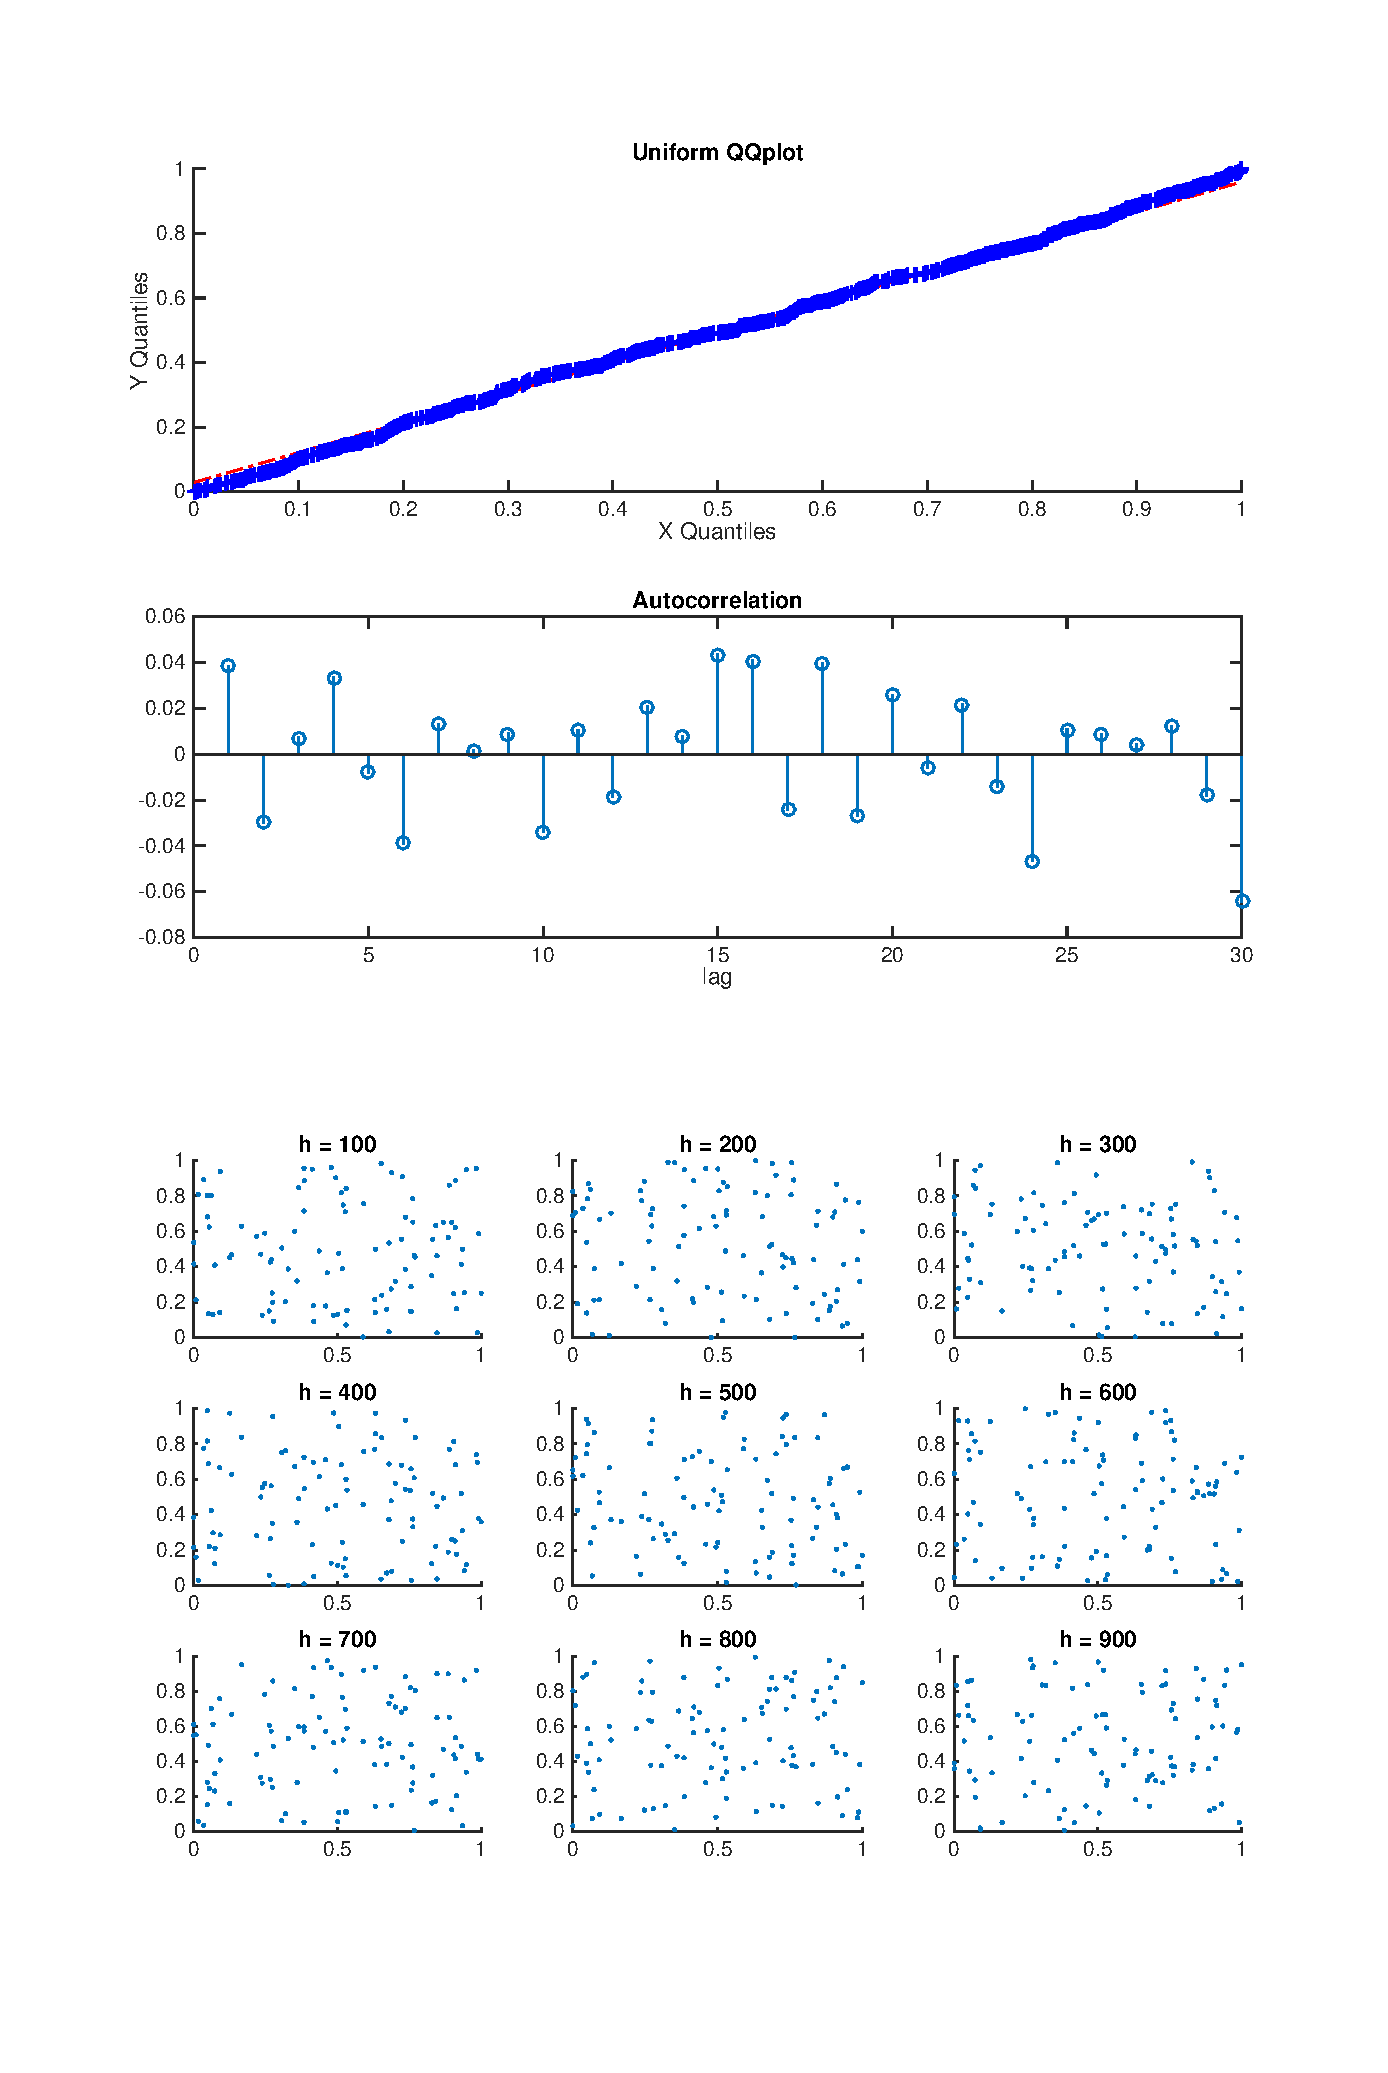
\includegraphics[width=0.7\textwidth]{images/hw2_1_65}
  \caption{Figure 6.5 in \cite{leb}}
  \label{fig:65}
\end{figure}

A LCG however must be handled carefully when dealing with parallel streams. In Figure~\ref{fig:67} there are two lag plots at lag 1 which show that the behavior of a LCG depends on the initial seed. If the two seeds depend one on the other or are not randomly chosen, for example with entropy extraction, as in the first plot where $x_0^{\text{LGC}_1} = 1$ and $x_0^{\text{LGC}_2} = 2$, then there's a strong correlation between the two streams (actually up to the wrap around $x_i^{\text{LGC}_2} = 2x_i^{\text{LGC}_1}$). Instead, if the seed of the second stream is the last element of the first sequence and the total number of samples generated doesn't exceed the period of the LCG then the two sequences are uncorrelated.
\begin{figure}
  \centering
  \subfigure{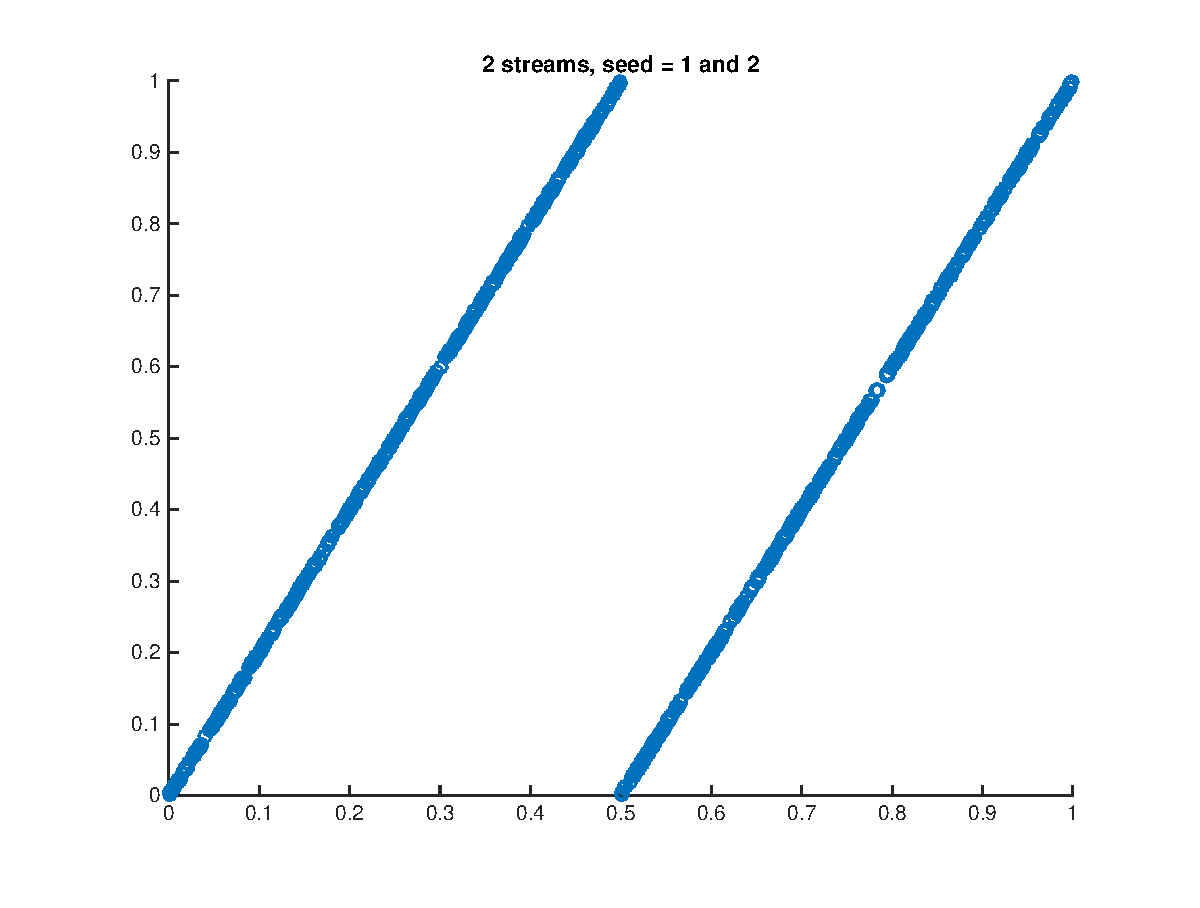
\includegraphics[width=0.7\textwidth]{images/hw2_1_67a}}
  \subfigure{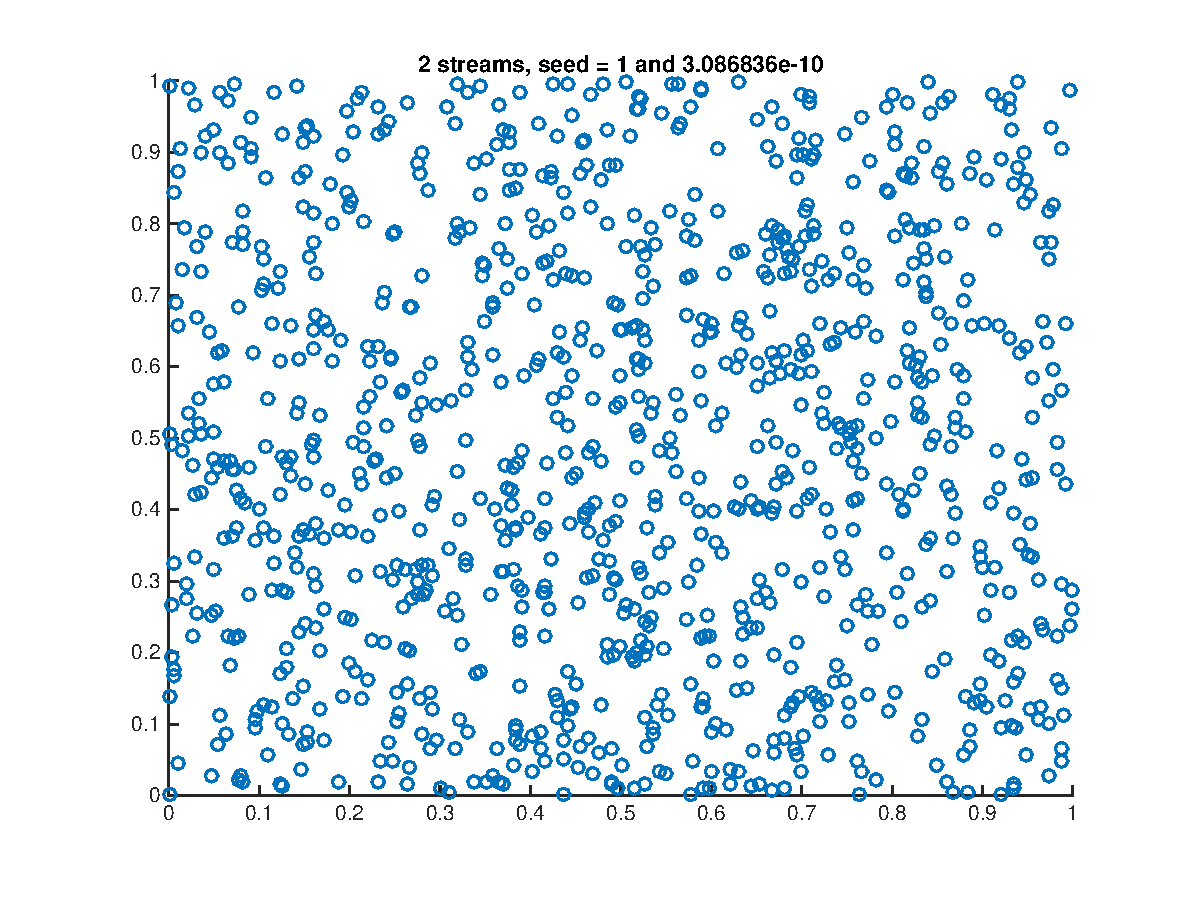
\includegraphics[width=0.7\textwidth]{images/hw2_1_67b}}
  \caption{Figure 6.7 in \cite{leb}}
  \label{fig:67}
\end{figure}

In Figure~\ref{fig:610} there are two distributions generated with rejection sampling. This technique allows to compute a random variable with a certain probability density distribution which is not completely known (i.e. missing normalization factor) by comparing uniform random variables with the expected values.
\begin{figure}
  \centering
  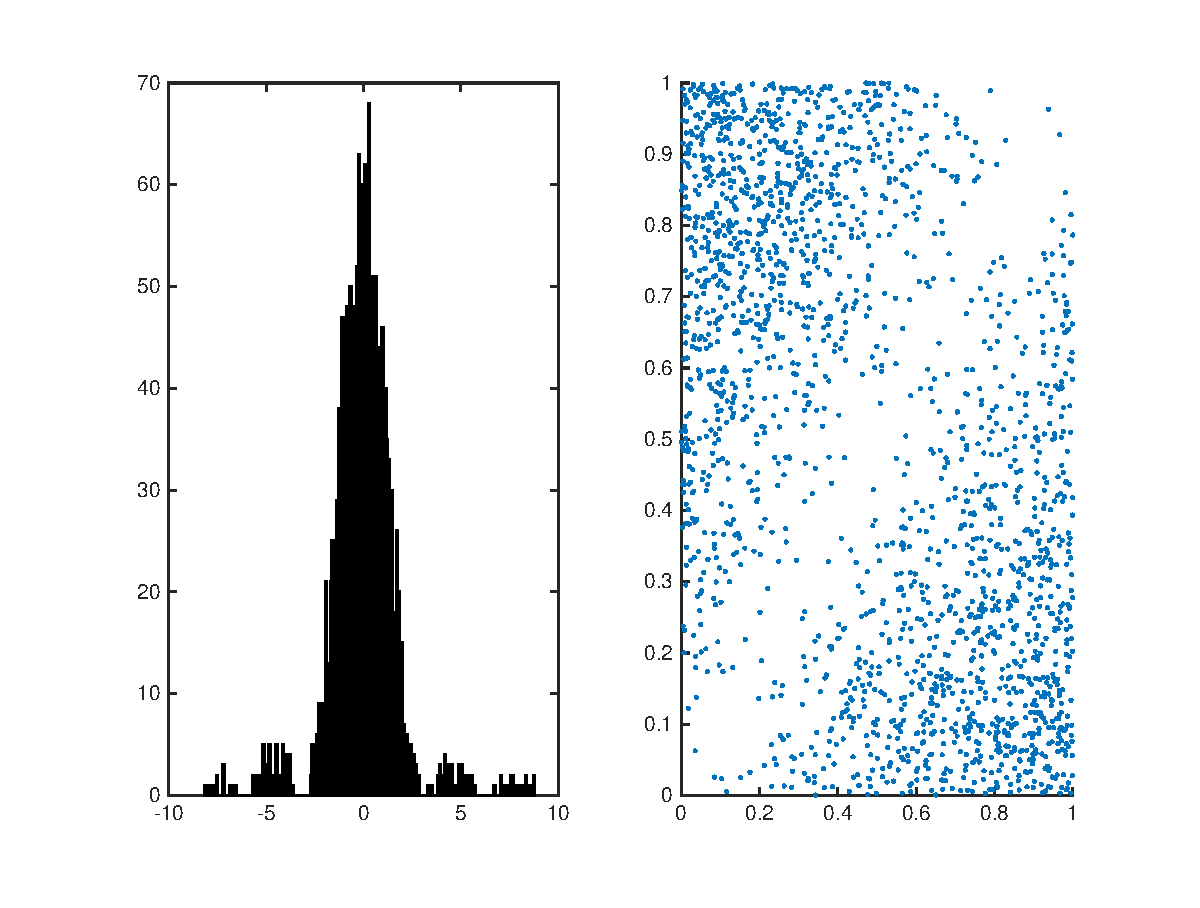
\includegraphics[width=0.7\textwidth]{images/hw2_1_610}
  \caption{Figure 6.10 in \cite{leb}}
  \label{fig:610}
\end{figure}

\section{Exercise 2}
A Binomial random variable (Bin($n, p$)) can be generated in three different ways. The first is the CDF inversion, which can be computed in an iterative way. Since the CDF of a Bin($n, p$) is $F(r) = \sum_{k = 0}^{r} \frac{n!}{(n-k)!k!} (1-p)^{n-k} p^k$ cannot be inverted in a close form, it is possible to compute it in an iterative way with the following algorithm:

\begin{algorithm}
  \caption{CDF inversion for Bin($n, p$)}\label{cdfinvbin}
  \begin{algorithmic}[1]
    \Procedure{}{}
    \State Let $U$ be a number, generated from a $U[0,1]$ distribution
    \State Let $X = 0, pr = (1-p)^n, F = pr, i = 0$
    \While {$U >= F$}
    \State $X = X + 1$
    \State $pr = \frac{n-i}{i+1} \frac{p}{1-p} pr$
    \State $F = F + pr$
    \State $i = i + 1$
    \EndWhile
    \State return $X$
    \EndProcedure
  \end{algorithmic}
\end{algorithm}

The second algorithm exploits the nature of the binomial distribution, which represents the number of success in $n$ Bernoulli trials with probability of success $p$. Therefore

\begin{algorithm}
  \caption{Generation of a Bin($n, p$) with $n$ bernoulli trials}\label{ber}
  \begin{algorithmic}[1]
    \Procedure{}{}
    \State Let $X = 0, i = 1$
    \While {$ i \le n$}
    \State Let $U$ be a number, generated from a $U[0,1]$ distribution
    \If {$U <= p$}
    \State $X = X + 1$
    \EndIf
    \State $i = i + 1$
    \EndWhile
    \State return $X$
    \EndProcedure
  \end{algorithmic}
\end{algorithm}

A more efficient variant of this method involves the generation of strings of $0$ (unsuccessful Bernoulli trials with $P_{\text{succ}} = p$) followed by a $1$, which is the first successful Bernoulli trial. These strings are distributed according to a geometric random variable $G(p)$. A geometric random variable can be generated with CDF inversion in a closed form, using $G = \floor{\frac{\log(U)}{\log(1-p)}}$ with $U$ a uniform sample in $[0,1]$. Thus
\begin{algorithm}
  \caption{Generation of a Bin($n, p$) with geometric strings of $0$}\label{geo}
  \begin{algorithmic}[1]
    \Procedure{}{}
    \State Let $X = 0$
    \State Let $U$ be a number, generated from a $U[0,1]$ distribution
    \State Let $G = \floor{\frac{\log(U)}{\log(1-p)}}$ the length of a string of zeros
    \State Let $i = G + 1$ a string of $G$ zeros and a $1$
    \While {$ i \le n$}
    \State $X = X + 1$
    \State Let $U$ be a number, generated from a $U[0,1]$ distribution
    \State Let $G = \floor{\frac{\log(U)}{\log(1-p)}}$ the length of a string of zeros
    \State $i = i +G+ 1$
    \EndWhile
    \State return $X$
    \EndProcedure
  \end{algorithmic}
\end{algorithm}

The algorithms are implemented in the attached MATLAB code in order to compare their performances. Note that the average number of iterations for Algorithm~\ref{cdfbininv} has to perform is one more than the value of the random variable it generates, so on average $1 + np$. Algorithm~\ref{ber} instead performs always $n$ iterations. The generation of geometric strings of zeros has a complexity which is proportional to $np$ too, since on average the strings have $\frac{1-p}{p}$ zeros and a 1, thus are long $1/p$: therefore the number of iterations needed to reach $n$ are on average $\frac{n}{1/p} = np$ (the comparisons are $1+np$). \\
The $n$ Bernoulli trials method is the slowest, especially when $n$ grows. The relation between the three methods can be seen in Figure~\ref{fig:bin}. CDF inversion and geometric method should perform approximately in the same way. Actually when there are many iterations the complex operations that Algorithm~\ref{geo} has to perform in each iteration (a logarithm, a division, an extraction of random number) make it slower that the simple CDF inversion. Instead when $np$ is small thus the number of iterations is on average lower than 1 then the two methods perform approximately in the same way. This can be seen in Figure~\ref{fig:bin_small} where it is plotted the time required to generate $10^5$ binomial random variables with $n\in [20, 10^4]$ (increased by a step of 20) and $p \in [10^{-9}, 10^{-8}, 10^{-7}, 10^{-6}, 10^{-5}]$.

This could actually be improved by looking at the values around the mean instead of beginning from 0. Note also that the CDF inversion method is based on iterations, thus the values it computes are subject to errors. Moreover it must be taken into account the limit of the finite precision of a computer, and since the lowest positive number which can be represented in MATLAB is $\delta = 4.9407e-324$ then for values of $n$ and $p$ such that $(1-p)^n < e$ the CDF inversion cannot be performed. This can happen for $p \approx 1/2$ and $n > 1000$.


\begin{figure}[h]
  \centering
  \subfigure[Bernoulli trials vs CDF inversion]{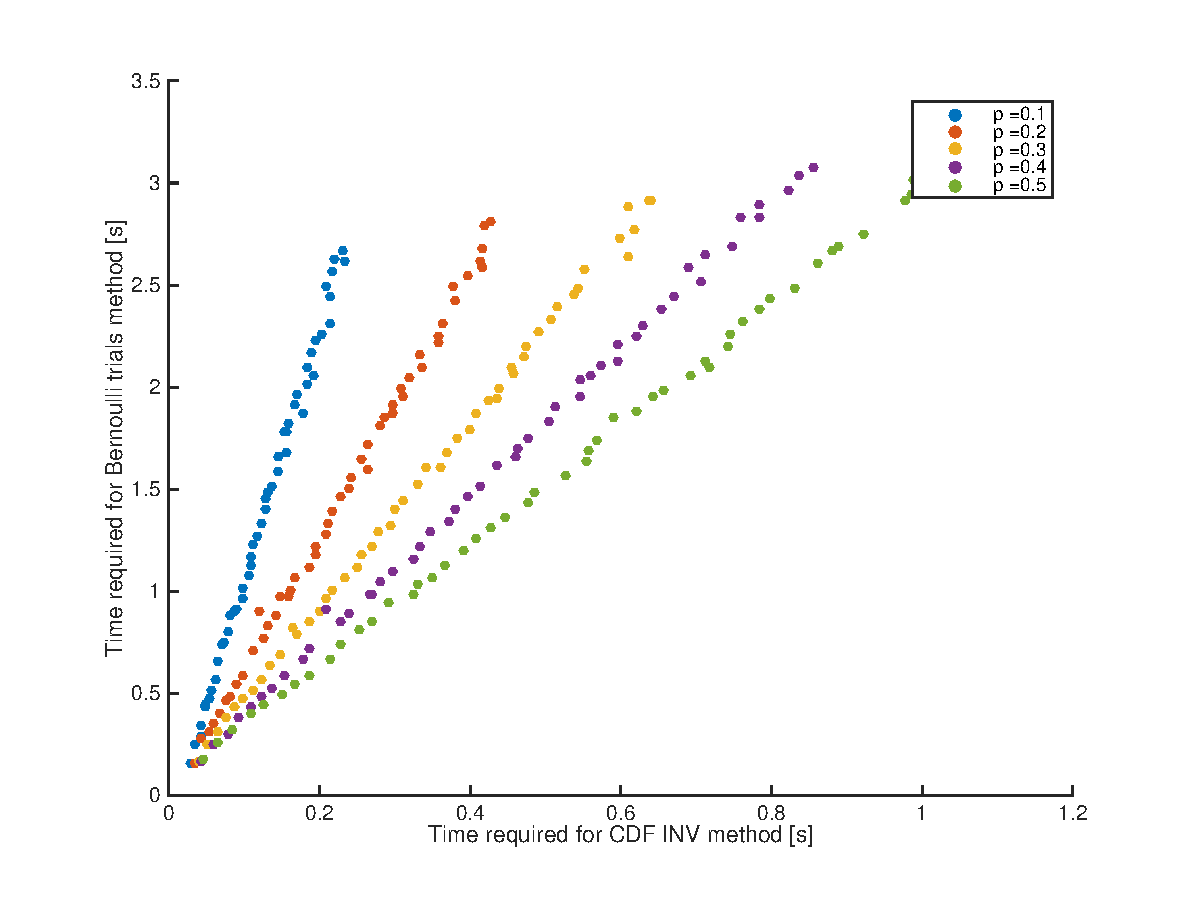
\includegraphics[width=0.45\textwidth]{images/inv_ber}}
  \subfigure[Bernoulli trials vs geometric strings]{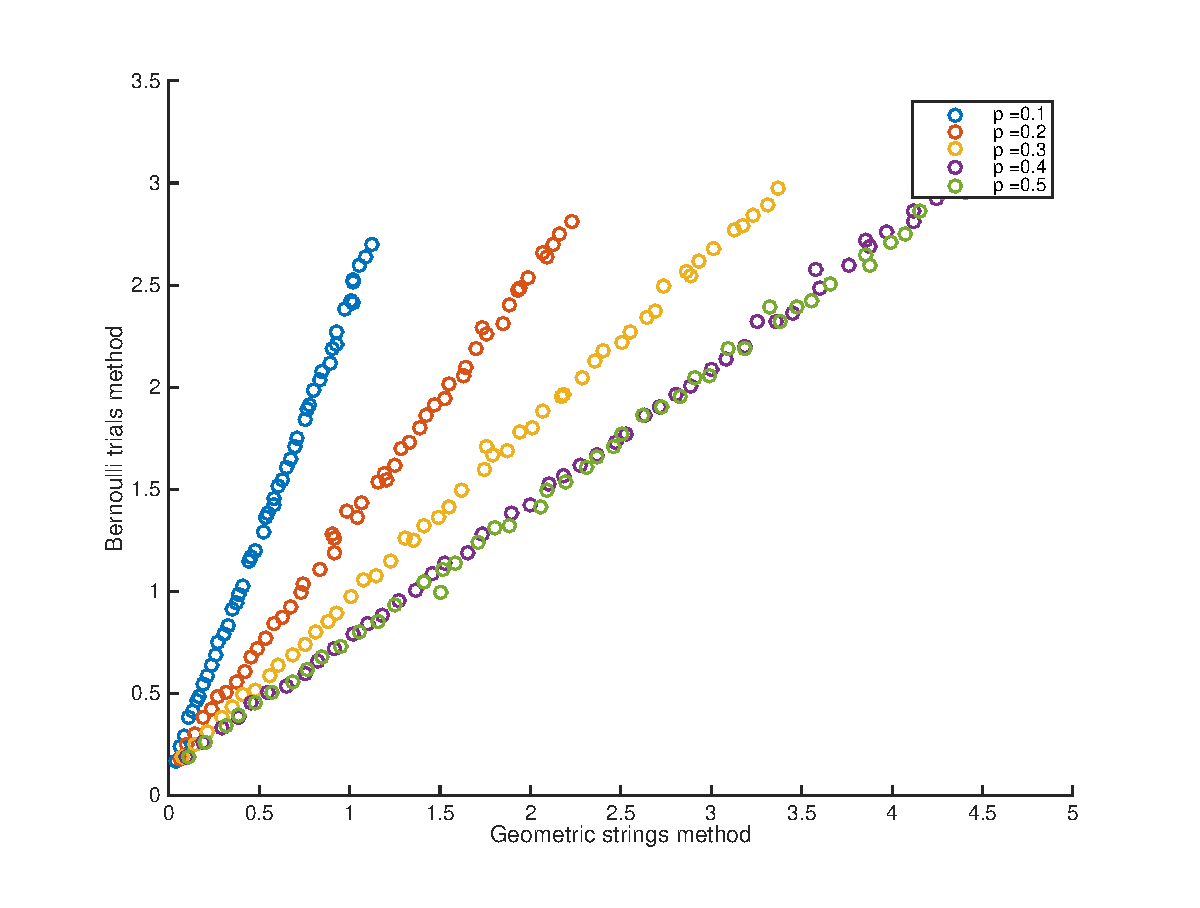
\includegraphics[width=0.45\textwidth]{images/geo_ber}}
  \subfigure[Geometric strings vs CDF inversion]{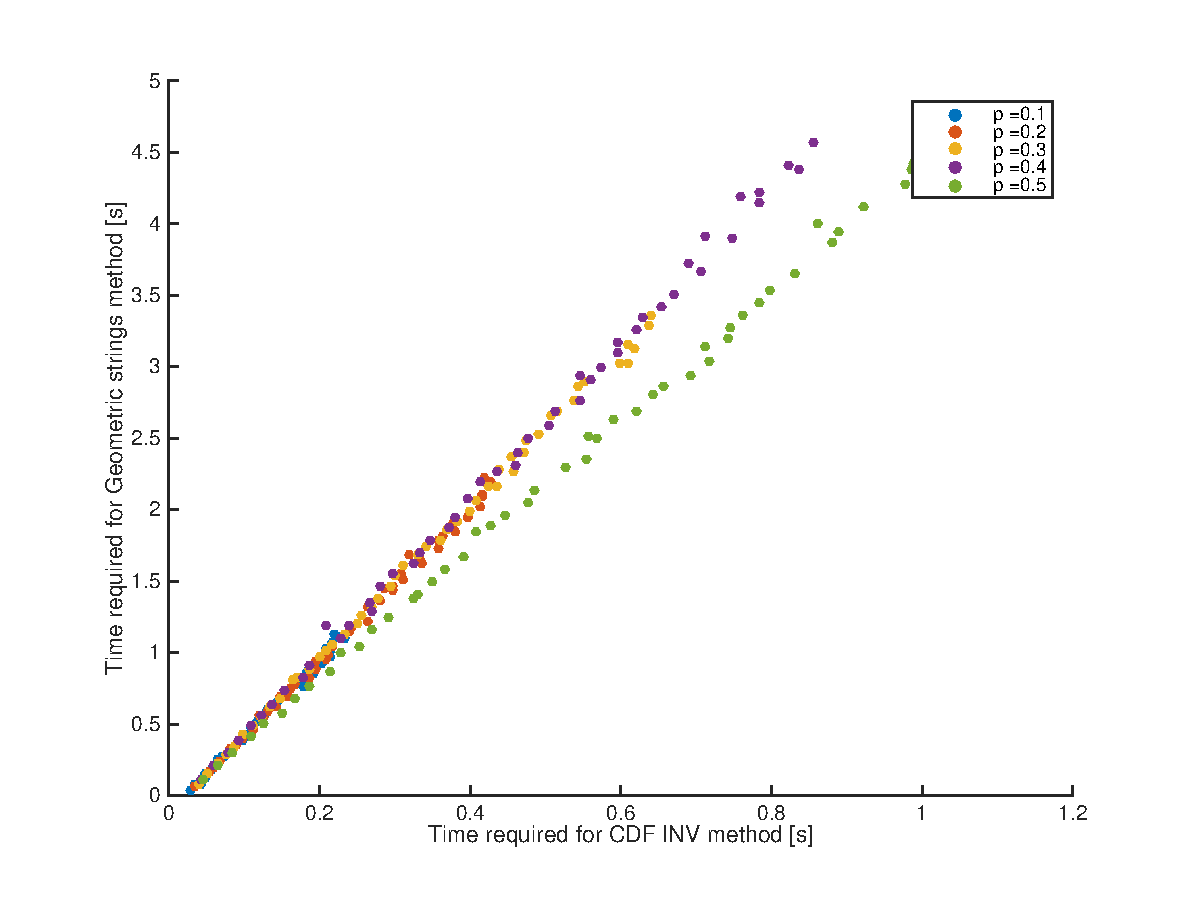
\includegraphics[width=0.45\textwidth]{images/inv_geo}}
  \caption{Comparison between time required to generate $N = 10^5$ binomial rv}
  \label{fig:bin}
\end{figure}

\begin{figure}[h]
  \centering
  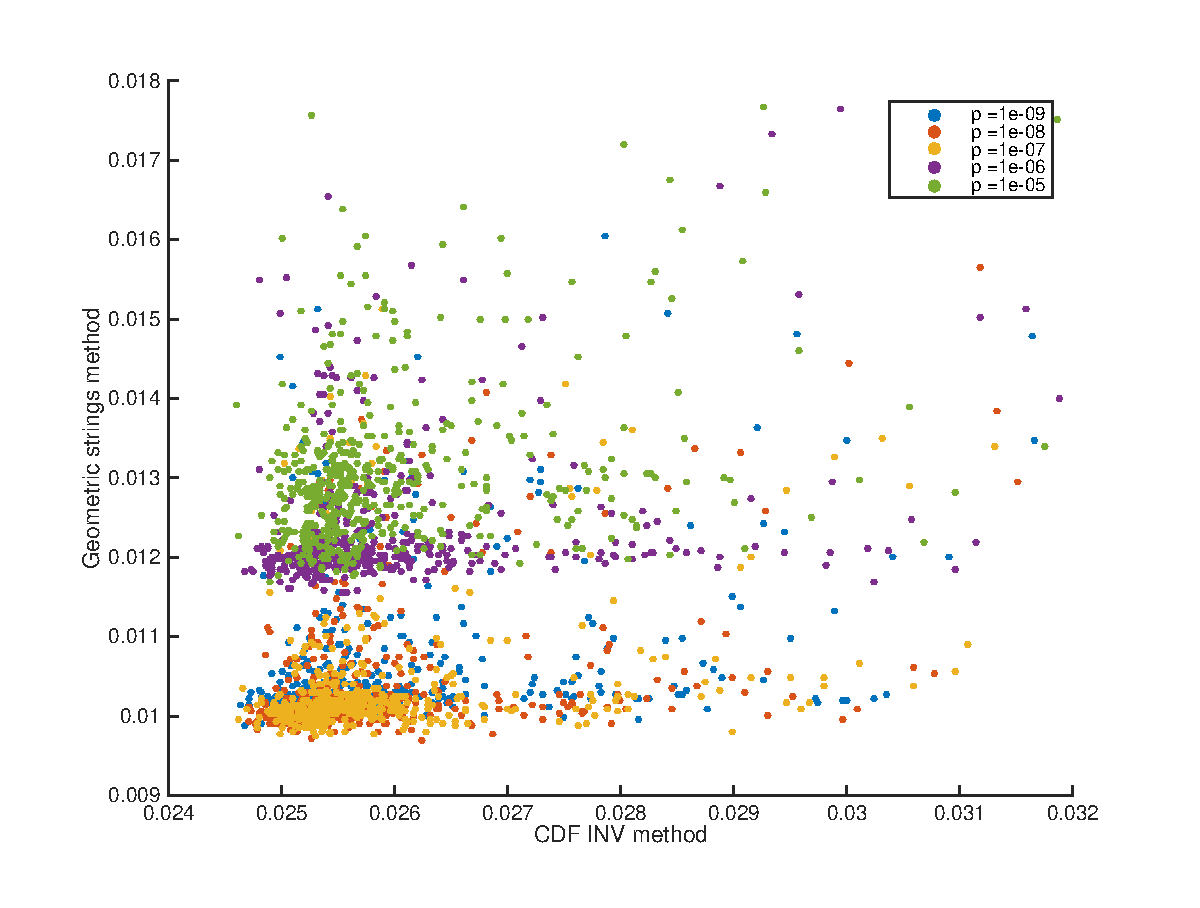
\includegraphics[width = 0.8\textwidth]{images/bin_smallp}
  \caption{Geometric strings vs CDF inversion methods' execution time for $np < 1$}
  \label{fig:bin_small}
\end{figure}


\section{Exercise 3}
A random variable which follows a Poisson distribution with parameter $\lambda$ can be generated in three ways: with CDF inversion (in an iterative fashion) and exploiting the property that link a Poisson distribution with the Poisson Process of intensity $\lambda$. \\
CDF inversion is performed in an iterative way. The CDF of a Poisson process is $F(k) = \sum_{i = 0}^k e^{-\lambda} \frac{\lambda ^i}{i!}$ and it can be written as $F(k+1) = \frac{\lambda}{k+1} F(k) + F(k)$ with $F(0) = e^{-\lambda}$. The following algorithm exploits this property:

\begin{algorithm}
  \caption{CDF inversion for Poisson($\lambda$)}\label{cdfinvpoi}
  \begin{algorithmic}[1]
    \Procedure{}{}
    \State Let $U$ be a number, generated from a $U[0,1]$ distribution
    \State Let $X = 0, pr = e^{-\lambda}, F = pr, i = 0$
    \While {$U >= F$}
    \State $X = X + 1$
    \State $pr = \frac{\lambda}{i+1}pr$
    \State $F = F + pr$
    \State $i = i + 1$
    \EndWhile
    \State return $X$
    \EndProcedure
  \end{algorithmic}
\end{algorithm}

The second algorithm is based on the following fact. In a Poisson process with intensity $\lambda$ the number of events in a time interval $t$ is distributed according to a Poisson distribution with mean $\lambda t$. The time between each event is an exponential with mean $\frac{1}{\lambda}$. The algorithm counts the number of events $X$ in a time interval $t=1$ by generating exponential random variables until they sum up to 1. The exact procedure is described in Algorithm~\ref{exp}. Note that an exponential random variable can be generated by the direct inversion of its CDF as like as the the geometric rv, using the formula $E = \frac{-1}{\lambda} \log(U)$ with $U$ a uniform $U[0,1]$ random variable.

\begin{algorithm}
  \caption{Generation of a Poisson($\lambda$) with exponential interarrival times}\label{exp}
  \begin{algorithmic}[1]
    \Procedure{}{}
    \State Let $X = 0$
    \State Let $U$ be a number, generated from a $U[0,1]$ distribution
    \State Let $E = \frac{-1}{\lambda} \log(U)$ the time of next event
    \State Let $i = E$ the time of last event
    \While {$ i \le 1$}
    \State $X = X + 1$
    \State Let $U$ be a number, generated from a $U[0,1]$ distribution
    \State Let $E = \frac{-1}{\lambda} \log(U)$
    \State $i = i + E$
    \EndWhile
    \State return $X$
    \EndProcedure
  \end{algorithmic}
\end{algorithm}

In the previous the Poisson random variable $X$ is defined as $X = \argmax_n{\sum_{i = 0}^n E_i \le 1}$ with $E_i = = \frac{-1}{\lambda} \log(U_i)$. Therefore $X = \argmax_n{\frac{-1}{\lambda} \sum_{i = 0}^n \log(U_i) \le 1} = \argmax_n{\frac{-1}{\lambda} \log( \Pi_{i = 0}^n U_i ) \le 1}$ and finally $X = \argmin_n \Pi_{i = 0}^n U_i > e^{-\lambda}$. Therefore the third algorithm is described by the following pseudocode.

\begin{algorithm}
  \caption{Generation of a Poisson($\lambda$) with product of uniforms}\label{prod}
  \begin{algorithmic}[1]
    \Procedure{}{}
    \State Let $X = 0$
    \State Let $U$ be a number, generated from a $U[0,1]$ distribution
    \State Let $i = U$
    \While {$ i \le e^{-\lambda}$}
    \State $X = X + 1$
    \State Let $U$ be a number, generated from a $U[0,1]$ distribution
    \State Let $i = Ui$
    \EndWhile
    \State return $X$
    \EndProcedure
  \end{algorithmic}
\end{algorithm}

All three methods have a computational complexity which is proportional to $\lambda$, as it can be seen in Figure~\ref{fig:poi_iter}. However the implementation of the third algorithm is much more expensive.

\begin{figure}[h]
  \centering
  \includegraphics[width = 0.8\textwidth]{images/poi_iter}
  \caption{Iterations required to generate $N = 1000$ Poisson random variables with the three methods}
  \label{fig:poi_iter}
\end{figure}

\begin{thebibliography}{10}

\bibitem{leb}
Y. Le Boudec, Performance Evaluation of Computer and Communications Systems, EPFL, 2015

\bibitem{pk}
M. Pinsky, S. Karlin, An Introduction to Stochastic Modeling, $4^{th}$ edition, Elsevier, 2011


\end{thebibliography}

\end{document}
